\subsubsection{向量平均}
由之前的介绍可知,词向量模型中,每个词都是一个高维向量,那么最简单直接的构造特征的方式就是将一段文本中所有词的词向量相加取平均,得到这段文本的平均词向量,将这个平均词向量作为该段文本的特征集合。\\
从直观角度理解,这种方式就是将一段文本的“重心”作为该段文本的特征。\\
利用这种特征来训练分类器,得到如下图\ref{fig:3cword2vecaverage}所示的ROC曲线。
\begin{figure}[h]
\centering
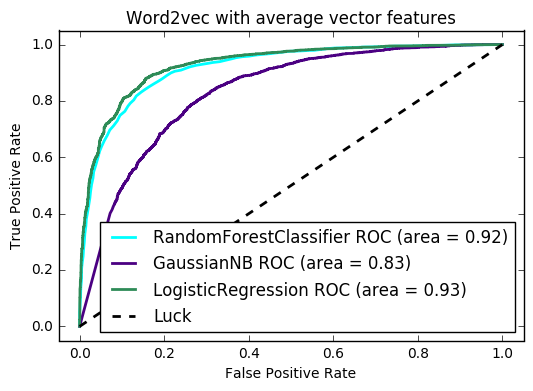
\includegraphics[width=0.9\linewidth]{3c_word2vec_average}
\caption[word2vec_average]{三种模型用Word2vec的平均词向量特征的ROC曲线}
\label{fig:3cword2vecaverage}
\end{figure}
用这个结果和简单词包的图4比较,发现在误差允许范围内,这种方式对结果并没有什么提高。\\
猜测原因是因为词向量虽然提供了文本的语义信息,但是却丢失了文本的统计信息。
从这个结果可以看出,词向量特征和词包特征是一对互补的特征,前者提供了语义信息,后者提供了统计信息。\\